%%%%%%%% CSCI 567 PROJECT FINAL REPORT %%%%%%%%%%%%%%%%%
%%%%%%%% Adapted from the ICML 2021 EXAMPLE LATEX SUBMISSION FILE %%%%%%%%%%%%%%%%%

\documentclass{article}

\usepackage{microtype}
\usepackage{graphicx}
\usepackage{subfigure}
\usepackage{booktabs}
\usepackage{amsmath}
\usepackage{hyperref}
\hypersetup{
  pdftitle={Row-Level Machine Learning for California Wildfire Occurrence Prediction Using Daily Weather and Seasonal Features},
  pdfauthor={Demy Brati, Calvin Kwong, Cheonhong (Jun) Lee, Matthew Montoya},
  pdfsubject={CSCI 567 Machine Learning Course Project},
  pdfkeywords={wildfire prediction, machine learning, row-level classification, California}
}

\newcommand{\theHalgorithm}{\arabic{algorithm}}

\usepackage[accepted]{icml2021}
% Suppress the ICML conference notice while keeping the course template style.
\makeatletter
\renewcommand{\Notice@String}{}
\makeatother

\begin{document}

\twocolumn[
\icmltitle{Row-Level Machine Learning for California Wildfire Occurrence Prediction Using Daily Weather and Seasonal Features}

\begin{icmlauthorlist}
\icmlauthor{Demy Brati}{}
\icmlauthor{Calvin Kwong}{}
\icmlauthor{Cheonhong (Jun) Lee}{}
\icmlauthor{Matthew Montoya}{}
\end{icmlauthorlist}

\vskip 0.3in
]

\hypersetup{
  pdfsubject={CSCI 567 Machine Learning Course Project},
  pdfkeywords={wildfire prediction, machine learning, row-level classification, California}
}

\begin{abstract}
Wildfire occurrence prediction is an important machine learning task, but the statewide tabular dataset used here lacks the spatial identifiers needed to support location-specific temporal sequence modeling. We build a row-level daily wildfire occurrence benchmark using the California Weather and Fire Prediction Dataset, restricting the primary analysis to 1984--2023 after identifying an all-negative tail in 2024 and early 2025. After auditing the dataset structure and finding no stable location identifier, we revise an initial temporal-windowed formulation into a same-row daily classification task to avoid unsupported sequence assumptions. Using a chronological train/validation/test split of 1984--2017, 2018--2020, and 2021--2023, we compare a class-prior baseline, logistic regression, Random Forest, XGBoost, tuned tree models, and a row-level multilayer perceptron. XGBoost and tuned XGBoost achieve the strongest test PR-AUC of 0.7572, while tuned Random Forest achieves the highest test F1 of 0.7239 and lowest Brier score of 0.1653. Feature relevance and seasonal error analysis show that calendar timing, temperature, and lagged precipitation drive much of the signal, while off-season fire days remain the hardest cases.
\end{abstract}

\section{Introduction}

Wildfire prediction is a natural machine learning problem for California because fire occurrence depends on weather, seasonality, and environmental context, and because even coarse risk estimates can support preparedness and resource planning. The task is not simply to fit historical fire labels. A useful model should generalize to future years, where weather patterns and fire regimes may differ from earlier training periods. Exploratory temporal analysis of the dataset also showed that fire occurrence is not uniform across 1984--2023: annual fire rates, monthly fire rates, and seasonal concentration vary over time. This motivated chronological evaluation rather than random splitting.

The project is also a case study in how dataset structure determines the claims a model can support. Prior wildfire literature often motivates temporal histories and spatiotemporal architectures, but such models require observations that can be interpreted as a coherent sequence for a location or region. A statewide daily table can still contain strong temporal and seasonal patterns, but those patterns do not automatically imply that a temporal window is a valid same-location history. This distinction became the main methodological issue in the project.

Prior wildfire prediction work motivates both the model families and the data limitations considered here. California-specific studies have evaluated classical supervised models such as decision trees, Random Forests, neural networks, and boosted models for wildfire prediction \citep{pham2022california,hernandez2024centralvalley,hahs2024datadriven}. Other work uses richer spatial or spatiotemporal structure, such as local regression and spatial clustering \citep{xie2025spatiotemporal}. These studies support the general idea that weather and temporal context are useful, but they also highlight a key distinction: models that claim local temporal dynamics need location-resolved observations. The California Central Valley study of \citet{hernandez2024centralvalley}, for example, focuses on a more specific geographic area, while the spatiotemporal framework of \citet{xie2025spatiotemporal} explicitly builds local structure into the modeling pipeline. This project is intentionally narrower: it asks what can be learned from the released statewide daily table when evaluation is fixed chronologically and the final task is aligned with the available columns.

The dataset used in this project is a statewide daily weather/fire dataset rather than a location-resolved panel. This distinction became central to the final project scope. A central part of the project was a scope revision from an initial temporal-windowed formulation to a row-level one-day benchmark after auditing the structure of the dataset. The temporal-windowed formulation was motivated by related wildfire literature: each example combined multiple adjacent daily rows and predicted a future fire label. However, the available columns did not include a county, station, latitude/longitude, grid cell, or other stable location identifier. Therefore, adjacent rows cannot be interpreted as consecutive observations from the same location. The final row-level formulation treats each row as an independent daily observation and asks: how well can daily weather, seasonality, and dataset-provided lag features predict fire occurrence for that row?

The main contributions are a row-level one-day benchmark, a comparison of linear, tree-based, boosted, and row-level neural models under the same chronological split, and an analysis of whether feature-level insights from the temporal-windowed formulation remain consistent under the row-level formulation. The final report is organized around three research questions: whether the row-level task is learnable, which model families are most reliable under future-year evaluation, and whether the earlier temporal-windowed analysis produced feature-level intuition that survives the scope revision.

\section{Methods}

\subsection{Dataset and Row-Level Prediction Task}

The project uses the California Weather and Fire Prediction Dataset with engineered features \citep{yavas2025california}. The released file covers 1984 through early 2025. The 2024 and early-2025 portion of the project dataset contained 378 rows and no positive fire-start labels. To avoid treating a potentially incomplete recent period as true negative data, all primary experiments use observations through 2023 rather than allowing the evaluation to depend on a block with no recorded positives. The target is \texttt{FIRE\_START\_DAY}, a binary indicator for whether a fire start occurred on the daily observation. The raw dataset contains 14,988 rows and 14 columns. After adding a numeric season encoding for modeling, the prepared table contains 15 columns. Through 2023, the active analysis set contains 14,610 rows with a positive rate of 0.3402.

Table~\ref{tab:data_split} summarizes the row-level one-day benchmark. The final task is one-day classification: one daily row provides the input features, and the same row's fire-start label is the target. The dataset-provided lagged precipitation and wind columns are retained because they are released row-level columns, not features constructed by this project from adjacent rows. They are treated as part of the supplied engineered row representation; no additional rolling multi-row features are created for the final benchmark.

The final benchmark scope is important because the scope revision is methodological rather than cosmetic: it changes the unit of supervision rather than only changing implementation details. In the temporal-windowed formulation, a six-day input window implicitly treated adjacent daily rows as a local history for one prediction target. That assumption would be appropriate for a panel indexed by location and date, such as county-day or grid-cell-day observations. However, the dataset does not include a key that verifies whether rows at day $t-1$ and day $t$ describe the same local context. The row-level formulation therefore avoids creating examples whose validity depends on unobserved location continuity. Temporal information is still represented through calendar variables and the dataset-provided lagged weather columns described above, but the model is no longer asked to learn from manually constructed sequences that the data cannot justify. When feature relevance is compared later, temporal-windowed importances are collapsed back to base feature families rather than used as final sequence evidence.

\begin{table}[t]
\caption{Dataset and row-level evaluation setup.}
\label{tab:data_split}
\vskip 0.03in
\begin{center}
\begin{small}
\begin{tabular}{ll}
\toprule
Item & Value \\
\midrule
Released range & 1984-01-01 to 2025-01-12 \\
Analysis range & Through 2023 \\
Rows through 2023 & 14,610 \\
Target positive rate & 0.3402 \\
Location identifier & Not available \\
Train years & 1984--2017 \\
Validation years & 2018--2020 \\
Test years & 2021--2023 \\
Final task & Row-level one-day classification \\
\bottomrule
\end{tabular}
\end{small}
\end{center}
\vskip -0.24in
\end{table}

\subsection{Features and Splits}

The row-level feature set includes precipitation, maximum
and minimum temperature, average wind speed, temperature
range, wind-temperature ratio, month, day of year, season
encoding, lagged precipitation, and lagged average wind
speed. The variables \texttt{LAGGED\_PRECIPITATION} and
\texttt{LAGGED\_AVG\_WIND\_SPEED} are dataset-provided delayed
weather columns attached to each daily row, so they are treated as
row-level inputs rather than rolling features constructed by this
project. These features intentionally mix weather state, simple
derived weather interactions, and calendar position. Median imputation
is used for missing feature values. Logistic Regression and the MLP
additionally use standard scaling; Random Forest and XGBoost use the
imputed tabular values directly.

All experiments use the same chronological split. Models train on 1984--2017, thresholds and tuning choices are selected on 2018--2020, and final results are evaluated once on 2021--2023. The validation period has a higher positive rate than the training period, which makes PR-AUC and validation-selected thresholds important for interpreting the results.

The split is also useful for checking whether performance survives a realistic time shift. The training block has a fire-start rate of 0.3204, while the validation and test blocks have rates of 0.4808 and 0.4247, respectively. A random split would blur this temporal change and could make the task look easier by mixing future-year patterns into training. The chronological split is therefore not only a conservative evaluation choice; it is part of the project design.

\subsection{Models and Evaluation}

The model suite contains a naive class-prior baseline, Logistic Regression, Random Forest, XGBoost, tuned Random Forest, tuned XGBoost, and a selected row-level multilayer perceptron. The naive baseline provides a lower-bound reference for the chronological split, while Logistic Regression tests whether a linear decision boundary over the row-level features is already informative. Random Forest is included because it is a strong nonlinear tabular baseline and gives direct impurity-based feature importance \citep{breiman2001random}. XGBoost is included as a boosted tree comparator that often performs well on structured tabular data \citep{chen2016xgboost}. The selected MLP is a two-hidden-layer feed-forward network with 64 and 32 hidden units, ReLU activations, dropout regularization, AdamW optimization, and binary cross entropy with logits. Its architecture was selected from a bounded validation-only search over six feed-forward candidates, including one-layer and two-layer networks with different hidden widths and dropout rates. The \texttt{[64, 32]} architecture with dropout 0.30 in both hidden layers achieved the highest validation PR-AUC among candidates, so the held-out test years remained reserved for final evaluation rather than architecture selection. It is valid under the row-level formulation because it consumes a single feature vector rather than an ordered temporal sequence. LSTM and GRU models are omitted from the final Results section because their interpretation depends on ordered local histories that the dataset does not provide.

The model set is intentionally limited to families that answer distinct questions: linear signal, nonlinear tabular interactions, boosted tabular learning, and a row-level neural baseline. Tuning is included to distinguish a weak baseline from a poorly configured baseline, but all model selection remains validation-based.

Evaluation uses ROC-AUC, PR-AUC, precision, recall, and F1. ROC-AUC summarizes ranking quality over all thresholds, while PR-AUC is more informative about positive-class retrieval when the positive rate changes across time. F1 is reported at a single decision threshold because it reflects the thresholded classification setting. Thresholds are selected on the validation years only and then applied once to the held-out test years. This keeps the test period reserved for final evaluation rather than model selection.

\section{Results}

\subsection{Row-Level Model Performance}

Table~\ref{tab:model_results} gives the final row-level one-day results. Under the row-level formulation, the task remains learnable. Logistic Regression substantially improves over the naive baseline, which indicates that row-level weather and seasonal features contain meaningful signal. The strongest models form a tight cluster: XGBoost has the best test PR-AUC, tuned Random Forest has the highest test F1 among tree models, and the selected MLP has the highest validation PR-AUC while nearly matching XGBoost on held-out PR-AUC.

The size of the performance gap is important. The naive baseline reaches a test PR-AUC of 0.4247, matching the positive rate in the test block, while Logistic Regression increases test PR-AUC to 0.6899. This shows that the row-level features contain signal before using complex nonlinear models. The tree models then improve ranking quality to roughly 0.75 test PR-AUC. The selected MLP is competitive and nearly matches XGBoost on test PR-AUC, but it does not clearly dominate across the held-out metrics. The main result is therefore not that a larger model family solves the task; it is that the row-level representation already contains substantial predictive signal, and several nonlinear classifiers can extract it with similar effectiveness.

\begin{table}[t]
\caption{Row-level one-day model comparison. F1 uses thresholds selected on validation years only; ROC-AUC and PR-AUC are threshold-free. Bold values mark the best metric in each column; XGBoost and tuned XGBoost share the best test PR-AUC because the tuning search selected the base configuration.}
\label{tab:model_results}
\vskip 0.03in
\begin{center}
\begin{small}
\begin{tabular}{lcccc}
\toprule
Model & Val PR & Test ROC & Test PR & Test F1 \\
\midrule
Naive baseline & 0.4808 & 0.5000 & 0.4247 & 0.5962 \\
Logistic & 0.7929 & 0.7888 & 0.6899 & 0.7155 \\
Random Forest & 0.8125 & 0.8232 & 0.7413 & 0.7193 \\
XGBoost & 0.8377 & 0.8268 & \textbf{0.7572} & 0.7231 \\
Tuned RF & 0.8331 & \textbf{0.8311} & 0.7531 & \textbf{0.7239} \\
Tuned XGBoost & 0.8377 & 0.8268 & \textbf{0.7572} & 0.7231 \\
Selected MLP & \textbf{0.8412} & 0.8269 & 0.7563 & 0.7211 \\
\bottomrule
\end{tabular}
\end{small}
\end{center}
\vskip -0.14in
\end{table}

The tuned XGBoost search selected the same configuration as the base XGBoost run in the final comparison, so tuning did not materially improve XGBoost beyond the base configuration. This result is informative: it shows that the original XGBoost configuration was already strong and that additional tuning was not the source of the result. In contrast, tuning Random Forest slightly improved the held-out F1 and ROC-AUC relative to the untuned Random Forest. Calibration analysis adds context for the validation-selected thresholds: tuned Random Forest has the lowest Brier score among the calibrated final row-level models (0.1653), while the selected MLP is close behind (0.1669) and has a mean predicted probability nearly equal to the test positive rate. XGBoost and tuned XGBoost retain the strongest held-out PR-AUC. Figure~\ref{fig:model_comparison} shows the same conclusion visually: the nonlinear row-level models cluster closely, and the naive baseline is clearly separated from every learned model.

\begin{figure}[t]
\vskip 0.03in
\begin{center}
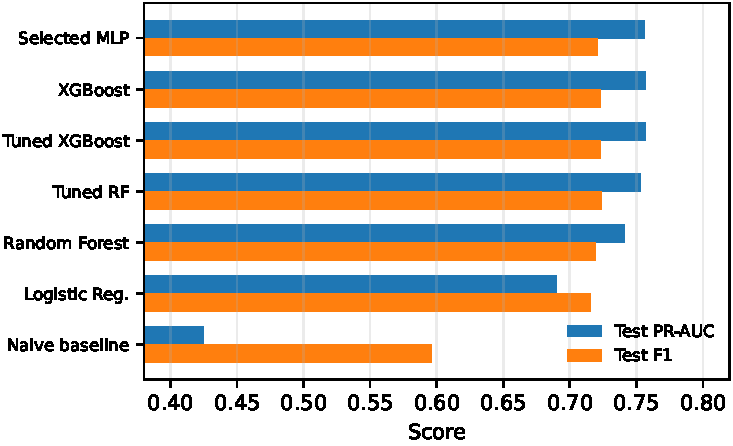
\includegraphics[width=\columnwidth]{figures/row_level_model_comparison.pdf}
\caption{Held-out performance for the final row-level model suite. Test PR-AUC and tuned test F1 show that XGBoost, tuned Random Forest, and the selected MLP are close rather than one model clearly dominating.}
\label{fig:model_comparison}
\end{center}
\vskip -0.22in
\end{figure}

\subsection{Feature Relevance}

Feature relevance supports the central interpretation that seasonality and temperature dominate the row-level task. Figure~\ref{fig:feature_diagnostics}(a) compares normalized row-level feature relevance against the aggregated feature relevance from the temporal-windowed formulation. The temporal-windowed formulation is not treated as a valid final forecasting setup, but its feature importances can be aggregated back to the base feature level and compared to the row-level model.

The aggregation step is what makes this comparison meaningful. The temporal-windowed formulation contains lag-specific copies of the row-level predictors and systematic 3\mbox{-}day, 7\mbox{-}day, and 14\mbox{-}day engineered summaries. Raw column importances are not directly comparable to the row-level feature set because one weather concept can appear through several lagged or summarized columns. We therefore aggregate temporal-windowed importances back to base feature families before comparison. Figure~\ref{fig:feature_diagnostics}(a) is therefore a feature-family comparison: it asks whether the two formulations emphasize similar underlying information, not whether an individual lagged or engineered column has the same interpretation as a row-level input.

\begin{figure*}[t]
\vskip 0.02in
\begin{center}
\subfigure[Feature-family comparison across formulations.]{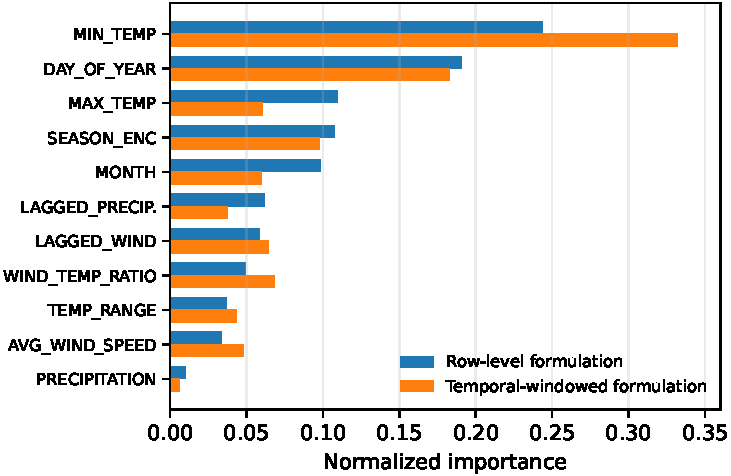
\includegraphics[width=0.48\textwidth]{figures/formulation_feature_relevance_comparison.pdf}}
\hfill
\subfigure[Validation permutation importance for the selected MLP.]{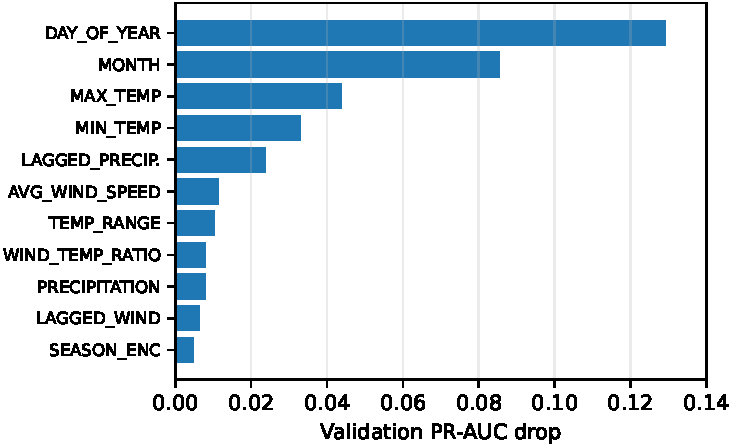
\includegraphics[width=0.48\textwidth]{figures/selected_mlp_permutation_importance.pdf}}
\caption{Feature relevance diagnostics. Panel (a) compares row-level feature relevance with temporal-windowed importances aggregated back to base feature families. Panel (b) shows validation permutation importance for the selected row-level MLP. Both diagnostics emphasize calendar position and temperature-related variables.}
\label{fig:feature_diagnostics}
\end{center}
\vskip -0.18in
\end{figure*}

This comparison focuses on feature-family agreement rather than treating the temporal-windowed formulation as a final forecasting method. Although the windowed design is not used for final predictive claims, both analyses identify minimum temperature, day of year, and seasonal variables as important. The row-level model also gives more relative weight to maximum temperature, month, and lagged precipitation. This shift is consistent with the row-level formulation: once manually constructed window positions are removed, the model relies more directly on same-row calendar position and weather state. The selected MLP's validation permutation importance follows the same pattern: day of year produces the largest PR-AUC drop when permuted, followed by month, maximum temperature, minimum temperature, and lagged precipitation. Figure~\ref{fig:feature_diagnostics}(b) reports this diagnostic. The use of validation data for permutation importance avoids using the test set to choose or interpret the final MLP.

Calendar dominance is meaningful but also limiting. A statewide daily dataset naturally contains strong month-of-year structure because fire starts are concentrated in particular seasons. This means a model can achieve strong aggregate performance by learning when fire starts are common, but it may still underreact to rare positives outside the dominant season. The weather variables help move the model beyond a pure seasonal prior, especially maximum temperature, minimum temperature, and lagged precipitation, but the feature relevance results show that the strongest signal remains a combination of calendar position and broad weather state.

The feature comparison also serves as a sanity check on the scope revision. If the temporal-windowed formulation had emphasized unrelated variables, the earlier exploratory results would be difficult to interpret. Instead, its strongest feature families overlap with the row-level formulation, especially temperature and calendar position. The difference is in what the comparison can support: it suggests that the exploratory formulation was detecting real aggregate seasonal and weather signal, not that the six-day input window represented a valid local trajectory. This distinction preserves a useful empirical insight while narrowing the final claims to what the dataset can support.

\subsection{Error Analysis}

The row-level error analysis uses the validation-selected XGBoost threshold, because XGBoost has the strongest held-out PR-AUC among the final models. The test-period confusion summary contains 410 true positives, 371 true negatives, 259 false positives, and 55 false negatives. These errors are not evenly distributed across seasons. As shown in Figure~\ref{fig:seasonal_errors}, the model almost always catches summer fire days, while winter fire days are much harder.

\begin{figure}[t]
\vskip -0.02in
\begin{center}
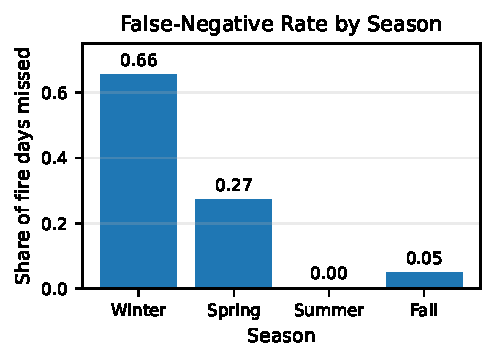
\includegraphics[width=\columnwidth]{figures/seasonal_error_analysis.pdf}
\caption{False-negative rate among true fire days in the row-level test set. The model is strongest during summer fire conditions and weakest on rare winter fire days.}
\label{fig:seasonal_errors}
\end{center}
\vskip -0.30in
\end{figure}

This pattern suggests that the models learn a strong seasonal prior. That improves overall performance because most fire days occur during the dominant fire season, but it also creates a limitation: unusual off-season fire starts remain difficult. This agrees with the dataset-level temporal analysis: fire occurrence is strongly structured by month and season, so a model can perform well overall while still struggling on rare off-season positives. The row-level formulation supports this conclusion without relying on unsupported temporal windows.

The seasonal breakdown also clarifies the precision-recall tradeoff behind the aggregate metrics. In the 2021--2023 test block, the model misses only 1 of 227 summer fire days, but misses 19 of 29 winter fire days and 30 of 110 spring fire days. Raising the threshold would reduce some false positives, especially during periods where the model predicts aggressively, but it would likely make rare off-season fire starts even harder to recover. This shows that the model's main weakness is distributional, not a random collection of isolated mistakes.


\section{Discussion and Limitations}

The results are best understood as a row-level occurrence benchmark rather than a deployed wildfire warning system or operational next-day forecast. The models predict whether a fire start is recorded for the same statewide daily observation; they do not predict ignition location, fire size, spread, suppression difficulty, or property exposure. Because the strongest predictors are seasonal and weather variables rather than local fuels or topography, location-resolved claims would require a different dataset.

The through-2023 cutoff is both a limitation and a methodological safeguard: it avoids treating a suspicious all-negative 2024 and early-2025 tail as reliable non-fire evidence, but it stops evaluation before the most recent fire seasons. The close performance among XGBoost, tuned Random Forest, and the selected MLP also argues against a claim that neural models clearly outperform tree ensembles. Most recoverable signal appears accessible to strong nonlinear tabular models; the MLP confirms that a bounded feed-forward neural baseline is competitive without changing the central conclusion.


\section{Process}

The project began with a broader wildfire-risk framing than the final benchmark. Wildfire prediction naturally suggests spatial location, fuels, topography, weather histories, and multiple forecast horizons, but combining those sources into a normalized machine learning table would require aligned spatial identifiers, temporal coverage, and feature definitions. The released dataset provided a usable statewide daily representation, so the first process challenge was auditing which claims that representation could support.

The initial modeling direction used a temporal-windowed formulation motivated by wildfire literature and dataset-level temporal patterns: each example concatenated daily features across a six-day input window and predicted a future fire label. The exploratory implementation included systematic 3\mbox{-}day, 7\mbox{-}day, and 14\mbox{-}day engineered summaries, multi-horizon labels, temporal robustness checks, advanced tabular models, and LSTM/GRU sequence models. It also identified annual fire-rate trends, monthly structure, feature autocorrelation, fire-day streaks, and seasonal error patterns.

Table~\ref{tab:scope_revision} summarizes the resulting scope revision. The important distinction is between aggregate temporal structure and supervised sequence validity. The exploratory analysis showed that fire labels and weather variables vary strongly over the calendar year and that some features are autocorrelated. Those findings explain why temporal modeling seemed reasonable, but they do not establish that adjacent rows form a valid same-location history for a sequence model.

\begin{table}[t]
\caption{Scope revision from temporal-windowed exploration to row-level modeling.}
\label{tab:scope_revision}
\vskip 0.03in
\begin{center}
\begin{scriptsize}
\setlength{\tabcolsep}{2pt}
\begin{tabular}{@{}p{0.22\columnwidth}p{0.35\columnwidth}p{0.35\columnwidth}@{}}
\toprule
Aspect & Temporal-windowed & Row-level \\
\midrule
Input unit & Six-day input window & One daily row \\
Target & Future fire label & Same-row fire-start label \\
Assumption & Local row continuity & Independent rows \\
Limitation & No location key & Matches available columns \\
Report role & Process and feature context & Primary results \\
\bottomrule
\end{tabular}
\end{scriptsize}
\end{center}
\vskip -0.14in
\end{table}

A later dataset audit changed the final interpretation: no stable location key meant consecutive rows could not be treated as a same-location history. The project was revised to row-level one-day prediction. The temporal-windowed work was not discarded; it informed the feature-relevance comparison and helped separate aggregate temporal structure from valid location-specific sequences.

Model selection introduced a second challenge after sequence models left the final Results section. The neural comparison needed to remain bounded and row-level, so the final MLP was selected through a small validation-only search over feed-forward architectures rather than an open-ended search over deeper models. This kept the neural baseline comparable to tabular models and avoided using test years to choose architecture or dropout. LSTM/GRU results are excluded because they require ordered local continuity that the dataset does not guarantee; the multi-horizon and sequence experiments remain process evidence for a reasonable literature-inspired direction, not final predictive claims.

\section{Contributions}

The submitted code implements the row-level wildfire occurrence pipeline: dataset audit, through-2023 filtering, chronological splitting, baseline classifiers, tuned tree ensembles, bounded MLP configuration search, validation-threshold tuning, feature relevance analysis, calibration diagnostics, and seasonal error analysis. The code submission also preserves the temporal-windowed exploratory analysis, including temporal EDA, systematic engineered temporal summaries, windowed baselines, horizon experiments, temporal robustness checks, advanced models, and sequence-model experiments. That material documents process and feature-relevance context; the row-level formulation remains the source of the reported predictive results.

The project uses Python, pandas, NumPy, scikit-learn \citep{pedregosa2011scikit}, XGBoost \citep{chen2016xgboost}, PyTorch \citep{paszke2019pytorch}, and matplotlib. The final code and data submission includes the two executable notebooks, the released dataset or dataset link, and Colab instructions for running the notebooks top-to-bottom. Saved CSV outputs allow report tables and figures to be regenerated without manual transcription. Code and dataset links are listed in Appendices~\ref{app:code} and~\ref{app:dataset}.

\section{AI Usage}

AI tools used during development included ChatGPT by OpenAI, GitHub Copilot by Microsoft, Qwen by Alibaba Cloud, and DeepSeek by High-Flyer. They supported brainstorming, code drafting and refinements, LaTeX formatting, English-language editing, spell checking, translation, and prose revision. Human review, technical judgment, and intuition developed through CSCI 567 guided the project direction, modeling scope, experiment selection, and final interpretation; the team ran the experiments, reviewed outputs, selected results, and is responsible for the final claims, results, code, and report.


\section{Conclusion}

California wildfire occurrence remains learnable under the row-level one-day benchmark, but no model family dominates: XGBoost and tuned XGBoost lead test PR-AUC, tuned Random Forest has the highest test F1 and lowest Brier score, and the selected MLP is competitive. Feature relevance and errors show that the main signal comes from seasonal timing, temperature, and lagged precipitation, while winter fire starts remain hardest. Future work should use location-indexed observations and geospatial covariates such as fuels, topography, fire perimeters, remote sensing, and gridded weather. Platforms such as Google Earth Engine and NASA FIRMS could support that extension \citep{gorelick2017gee,nasafirms}. With a location-indexed panel, temporal-windowed or recurrent models would have valid local histories.

\clearpage
\bibliography{main}
\bibliographystyle{icml2021}

\appendix

\section{Code}
\label{app:code}
TODO: insert final GitHub repository link.

\section{Dataset}
\label{app:dataset}
The dataset used in this project is the California Weather and Fire Prediction Dataset (1984--2025) with Engineered Features, available from Zenodo at:\\
\url{https://doi.org/10.5281/zenodo.14712845}

\section{Acknowledgements}
\label{app:acknowledgements}
We acknowledge the CSCI 567 course staff for providing the report template. The report uses the ICML 2021 \LaTeX{} style file, originally created by P. Langley and later modified by ICML template contributors including Terran Lane, Kristian Kersting, Prasad Tadepalli, Andrew Moore, Ricardo Silva, Sam Roweis, Kiri Wagstaff, Hal Daum\'e III, Christoph Sawade, Tobias Scheffer, Francesco Figari, Sanjoy Dasgupta, Fei Sha, Percy Liang, Daniel Roy, and Iain Murray.

\end{document}
